\section{Experiment=21: SolCx manufactured solution}

The SolCx benchmark computes the Stokes flow field of a fluid driven by spatial density 
variations, subject to a spatially variable viscosity. Specifically, the domain 
is $\Omega = [0,1]^2$, gravity is $\vec{g} = (0,-1)^T$ and the density is given by  
\begin{equation}
\rho(x,y) = \sin(\pi y) \cos(\pi x)
\end{equation}
Boundary conditions are free slip on all of the sides of the domain and the 
temperature plays no role in this benchmark. 
The viscosity is prescribed as follows:
\begin{equation}
\eta(x,y) = 
\left\{
\begin{array}{lll}
1 & \text{for} & x<0.5 \\
10^6 & \text{for} & x>0.5 \\
\end{array}
\right.
\end{equation}
Note the strongly discontinuous viscosity field yields a stagnant flow 
in the right half of the domain and thereby yields a pressure discontinuity along the interface. 

Note that the source code which evaluates the velocity and pressure fields for both SolCx and SolKz is  
distributed as part of the open source package Underworld 
(\cite{moql07}, \url{https://www.underworldcode.org/intro-to-underworld/}).
I have translated this code to python. 

I first solve the linear system with the Uzawa3 solver, coming from
\cite{}. Since it does not implement any kind of preconditioning
its convergence is somewhat chaotic:

\begin{center}

\includegraphics[width=5.7cm]{exp21/uzawa3/solver_convergence_xiV.pdf}

\includegraphics[width=5.7cm]{exp21/uzawa3/solver_convergence_xiP.pdf}

\includegraphics[width=5.7cm]{exp21/uzawa3/solver_convergence_alpha.pdf}
\end{center}

Turning now to the cd-u-eta solver, we find that the number of
iterations is much smaller and the convergence monotonous:

\begin{center}

\includegraphics[width=5.7cm]{exp21/solver_convergence_xiV.pdf}

\includegraphics[width=5.7cm]{exp21/solver_convergence_xiP.pdf}\\

\includegraphics[width=5.7cm]{exp21/solver_convergence_alpha.pdf}
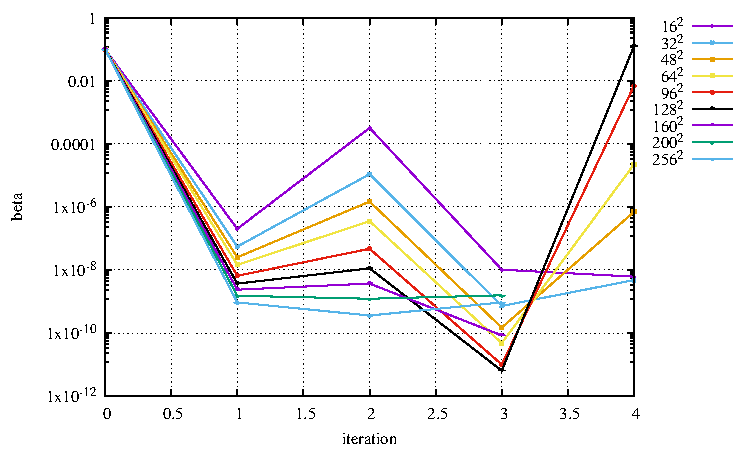
\includegraphics[width=5.7cm]{exp21/solver_convergence_beta.pdf}
\end{center}

As observed for example in \cite{thba22} the pressure 
convergence rate is only 0.5 because of the pressure discontinuity 
in the middle of the domain: 

\begin{center}

\includegraphics[width=7cm]{exp21/errors.pdf}
\end{center}

\newpage
\begin{center}

\includegraphics[width=5cm]{exp21/plt/solution_divv_0000.png}

\includegraphics[width=5cm]{exp21/plt/solution_e_0000.png}

\includegraphics[width=5cm]{exp21/plt/solution_eta_0000.png}\\

\includegraphics[width=5cm]{exp21/plt/solution_exx_0000.png}

\includegraphics[width=5cm]{exp21/plt/solution_exz_0000.png}

\includegraphics[width=5cm]{exp21/plt/solution_ezz_0000.png}\\

\includegraphics[width=5cm]{exp21/plt/solution_p_0000.png}

\includegraphics[width=5cm]{exp21/plt/solution_rho_0000.png}

\includegraphics[width=5cm]{exp21/plt/solution_u_0000.png}\\

\includegraphics[width=5cm]{exp21/plt/solution_vel_0000.png}

\includegraphics[width=5cm]{exp21/plt/solution_w_0000.png}
\end{center}

